\documentclass[a4paper]{article}
\usepackage[margin=7mm,top=8mm,bottom=7mm]{geometry}
\usepackage{graphicx}
\usepackage{xcolor}
\definecolor{cutgray}{gray}{0.35}
\usepackage{tikz}
\usepackage{array}
\pagestyle{empty}
\setlength{\parindent}{0pt}
\setlength{\parskip}{0pt}
\setlength{\tabcolsep}{1.2mm}
\renewcommand{\arraystretch}{1.0}

% Fixed grid: 2 x 3 cards per page for easy scissors cutting
\newcommand{\cardw}{94mm}
\newcommand{\cardh}{74mm}

% Draw cut frame around a pre-sized includegraphics
\newcommand{\portaltile}[1]{%
  \begin{tikzpicture}
    \node[inner sep=0pt, outer sep=0pt] (card) at (0,0)
      {\includegraphics[width=\cardw, height=\cardh, keepaspectratio=false]{#1}};
    \draw[cutgray, dashed, line width=0.7pt]
      (card.south west) rectangle (card.north east);
    \draw[black, line width=0.9pt]
      (card.south west) -- ++(0,3.2mm)
      (card.south west) -- ++(3.2mm,0)
      (card.south east) -- ++(0,3.2mm)
      (card.south east) -- ++(-3.2mm,0)
      (card.north west) -- ++(0,-3.2mm)
      (card.north west) -- ++(3.2mm,0)
      (card.north east) -- ++(0,-3.2mm)
      (card.north east) -- ++(-3.2mm,0);
  \end{tikzpicture}%
}

\begin{document}
\centering
{\large\bfseries Portal Address Tiles}\\[0.3mm]
{\footnotesize Hieroglyphs only. Bird faces the \emph{start} of the address. Cut on dashed lines. B/W laser OK.}\\[1.2mm]
\begin{tabular}{@{}c@{\hspace{2mm}}c@{}}
% Osireion (Abydos) / OSIREION / LTR
\portaltile{HieroGlyphs/tiles/abydos_osireion.png} &
% Boat Pits / BOATPITS / RTL
\portaltile{HieroGlyphs/tiles/boat_pits.png} \\[1.0mm]
% Builders' Quarters / BUILDERS / LTR
\portaltile{HieroGlyphs/tiles/builders_quarters.png} &
% Dendera Temple / DENDERA / RTL
\portaltile{HieroGlyphs/tiles/dendera_temple.png} \\[1.0mm]
% Eastern Cemetery / EASTCEM / LTR
\portaltile{HieroGlyphs/tiles/east_cemetery.png} &
% Eridu Ruins / ERIDU / RTL
\portaltile{HieroGlyphs/tiles/eridu_ruins.png} \\
\end{tabular}
\newpage
\centering
\begin{tabular}{@{}c@{\hspace{2mm}}c@{}}
% Underground Repository of Knowledge (Giza) / LIBRARY / LTR
\portaltile{HieroGlyphs/tiles/giza_repository.png} &
% Queen Hetepheres' Tombs / HETEPH / RTL
\portaltile{HieroGlyphs/tiles/hetepheres_tombs.png} \\[1.0mm]
% Inka Stone Door (Andes) / ANDES / LTR
\portaltile{HieroGlyphs/tiles/inka_andes.png} &
% Ancient Ziggurat (Iran) / ZIGGURAT / RTL
\portaltile{HieroGlyphs/tiles/iran_ziggurat.png} \\[1.0mm]
% Face Mountain (Mars) / MARS / LTR
\portaltile{HieroGlyphs/tiles/mars_face_mountain.png} &
% Sunken Giza Clone (Atlantic) / OCEAN / RTL
\portaltile{HieroGlyphs/tiles/ocean_giza_clone.png} \\
\end{tabular}
\newpage
\centering
\begin{tabular}{@{}c@{\hspace{2mm}}c@{}}
% Office of Pyramid Studies / OFFICE / LTR
\portaltile{HieroGlyphs/tiles/office_pyramid_studies.png} &
% Tomb of Queen Khentkawes / KHENT / RTL
\portaltile{HieroGlyphs/tiles/queen_khentkawes.png} \\[1.0mm]
% Rock Cut Tombs (Khafre) / ROCKCUT / LTR
\portaltile{HieroGlyphs/tiles/rock_cut_tombs_khafre.png} &
% Step Pyramid Complex (Saqqara) / SAQQARA / RTL
\portaltile{HieroGlyphs/tiles/saqqara_step_pyramid.png} \\[1.0mm]
% The Great Sphinx / SPHINX / LTR
\portaltile{HieroGlyphs/tiles/sphinx.png} &
% Sphinx's Shadow Chamber / SHADOW / RTL
\portaltile{HieroGlyphs/tiles/sphinx_shadow_chamber.png} \\
\end{tabular}
\newpage
\centering
\begin{tabular}{@{}c@{\hspace{2mm}}c@{}}
% Valley Temple of Khafre / VALLEYK / LTR
\portaltile{HieroGlyphs/tiles/valley_khafre.png} &
% Valley of the Queens / QUEENS / RTL
\portaltile{HieroGlyphs/tiles/valley_queens.png} \\[1.0mm]
% Western Cemetery / WESTCEM / LTR
\portaltile{HieroGlyphs/tiles/western_cemetery.png} & \\
\end{tabular}

\newpage
\centering
{\Large\bfseries Reading guide (players)}\\[1.5mm]
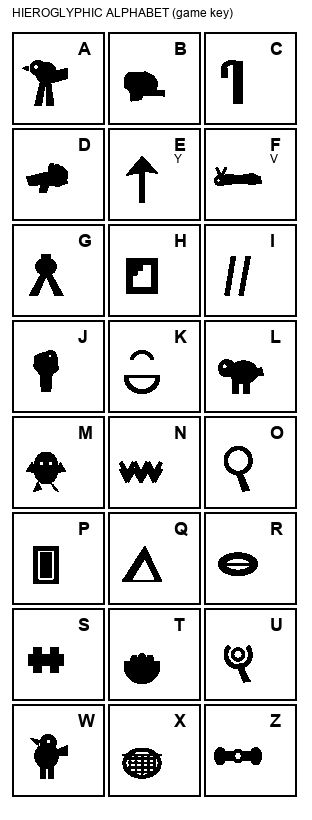
\includegraphics[height=0.72\textheight,keepaspectratio]{HieroGlyphs/alphabet_print_key.png}\\[2mm]
\begin{minipage}{0.92\textwidth}
\small
\begin{itemize}
  \item The \textbf{bird faces the beginning} of the address line.
  \item Bird faces \textbf{left} $\Rightarrow$ read \textbf{left-to-right}.
  \item Bird faces \textbf{right} $\Rightarrow$ read \textbf{right-to-left}
        (glyphs are already ordered for that direction --- start at the bird and read along the line).
  \item Match each symbol to this key \textbf{or} your wood papyrus from Egypt.
  \item Shared souvenir cells: \textbf{Y} uses \textbf{E}; \textbf{V} uses \textbf{F}.
\end{itemize}
\end{minipage}
\end{document}
